\chapter{Introduction}
%- INTRODUZIONE DELLA TESI E DEL LAVORO DI DOTTORATO (VEDI FIL)

%% FILTRARE LA SEGUENTE INTRODUZIONE (CSUR18) 
Nowadays, the amount of public available information encourages the study and development of algorithms that analyse huge amount of users' data with the aim to infer reactions about topics, opinions, trends and to understand the mood of the users whose produce and share information through the web. The aim of Sentiment Analysis is to extract the attitude of people toward a topic or the intended emotional affect the author wishes to have on the readers. The tasks of this research field are challenging as well as very useful in practice. Sentiment analysis finds several practical applications, since opinions influence many human decisions either in business and social activities.  

Sentiment analysis systems are being applied in almost every business and social domain because opinions are central to almost all human activities and are key influencers of our behaviours. 
Although NLP (Natural Language Processing) offers several approaches to address the problem of understanding users' preferences and behaviours, the social media context offers some additional challenges. Beside the huge amounts of available data, typically the textual communications on social networks consist of short and colloquial messages. Moreover, people tend to use also images and videos, in addition to the textual messages, to express their experiences through the most common social platforms.
The information contained in such visual contents are not only related to semantic information such as objects or actions about the acquired picture, but also cues about affect and sentiment conveyed by the depicted scene. Such information is hence useful to understand the emotional impact (i.e., the evoked sentiment) beyond the semantic.
For these reasons images and videos have become one of the most popular media by which people express their emotions and share their experiences in the social networks, which have assumed a crucial role in collecting data about people's opinions and feelings. 
Images and videos produced by users and shared in social media platforms reflect visual aspects of users' daily activities and interests. Such growing user generated images represent a recent and powerful source of information useful to analyse users' interests. 
%Extracting the emotions inherently underlying images perceived by the viewers could promote new approaches to several application fields such as brand perception, assessment of customer satisfaction, advertising, and media analytic, etc.
%The diffusion of personal mobile devices constantly connected to Internet services (e.g., smartphones) and the growth of social media platforms introduced a new communication paradigm by which people that share multimedia data. %, by allowing new interaction models. 
In this context, uploading images and videos to a social media platform is the new way by which people share their opinions and experiences.  
This provides a strong motivation for research on this field, and offers many challenging research problems.
This dissertation we present several scientific works that analyses images and videos produced by users in a social context (i.e., a social platform, a social event or a public site), with the aim to infer user's interests and behaviours.
The basic task in Visual Sentiment Analysis is the prediction of the sentiment evoked by a visual content (i.e., images and videos) in terms of sentiment polarity (i.e., positive, negative or neutral) or by using a set of emotion classes (i.e., angry, joy, sad, etc.).
In Section~\ref{secPolarity) we present our approach to the task of sentiment polarity prediction. After a deep revision of the state of the art, we address the challenge of image sentiment polarity by proposing a novel source of text for this task, dealing with the issue related to the use of text associated to images provided by users, which is commonly used in most of the previous works and is often noisy due its subjective nature.
However, in this dissertation we further extend the task of Sentiment Analysis applied to visual contents by considering the contribution of crowdsourced media. Indeed, beside the basic task of predicting the polarity of an image, the works presented in this thesis aim to perform inferences based on the analysis of sets of pictures/videos collected from specific groups of people with common interests. Thus, we defined several inference tasks, depending on the source media (photo or video) and the parameter to be predicted (sentiment or popularity). 
In Section~\ref{TSP} we present a framework that collects huge amount of photos taken from users during a specific period and place, with the aim to infer the behaviour of people visiting a cultural heritage site, or attending a specific event. All the inference are based on the photos taken by visitors, therefore this work highlights how shared pictures can reflect the users' behaviour and preferences.
Starting from the task of image popularity prediction, in Section~\ref{secPopularity} we define and present an even more challenging task, named popularity dynamics prediction. In this work we provide a description of the classic problem of predicting the popularity of an image and extend this task by adding the temporal axis. 
Then we present the first dataset related to this task and propose a solution to the temporal challenge.
In Chapter~\ref{ch4} we present our works on videos. In particular, Section\ref{RECfusion} presents a system that takes a set of videos recorded by different people in the same time and produces a unique video as output, by considering the most popular scenes over time, based on the number of people that are simultaneously paying attention to the same scene. This system is applied in public event contexts, such as concerts or public exhibitions, and implements an automatic selection of the scenes based on the preferences inferred from the users that are attending the event.
In Section~\ref{WearableRECfusion} we extend this approach in the context of personal context by proposing a system for the daily living activity monitoring for lifelogging.
%\\
%ALLARGARE LE CATEGORIE DI TASK, INSERENDO LE DIVERSE ACCEZIONI DI SENTIMENT 
%\\
%SENTIMENT  ---> CONTENT POLARITY AND CONTENT POPULARITY
%\\POLARITY   ---> POSITIVE / NEGATIVE EVOKED EMOTION ---> SENTIMENT PREDICTION
%\\POPULARITY ---> POPULARITY ON SOCIAL PLATFORMS --> FLICKR
%\\POPULARITY ---> POPULARITY IN SOCIAL EVENTS --> RECFUSION + TSP

\section{Dissertation Structure}
\begin{figure}[t]
	\centering
	%	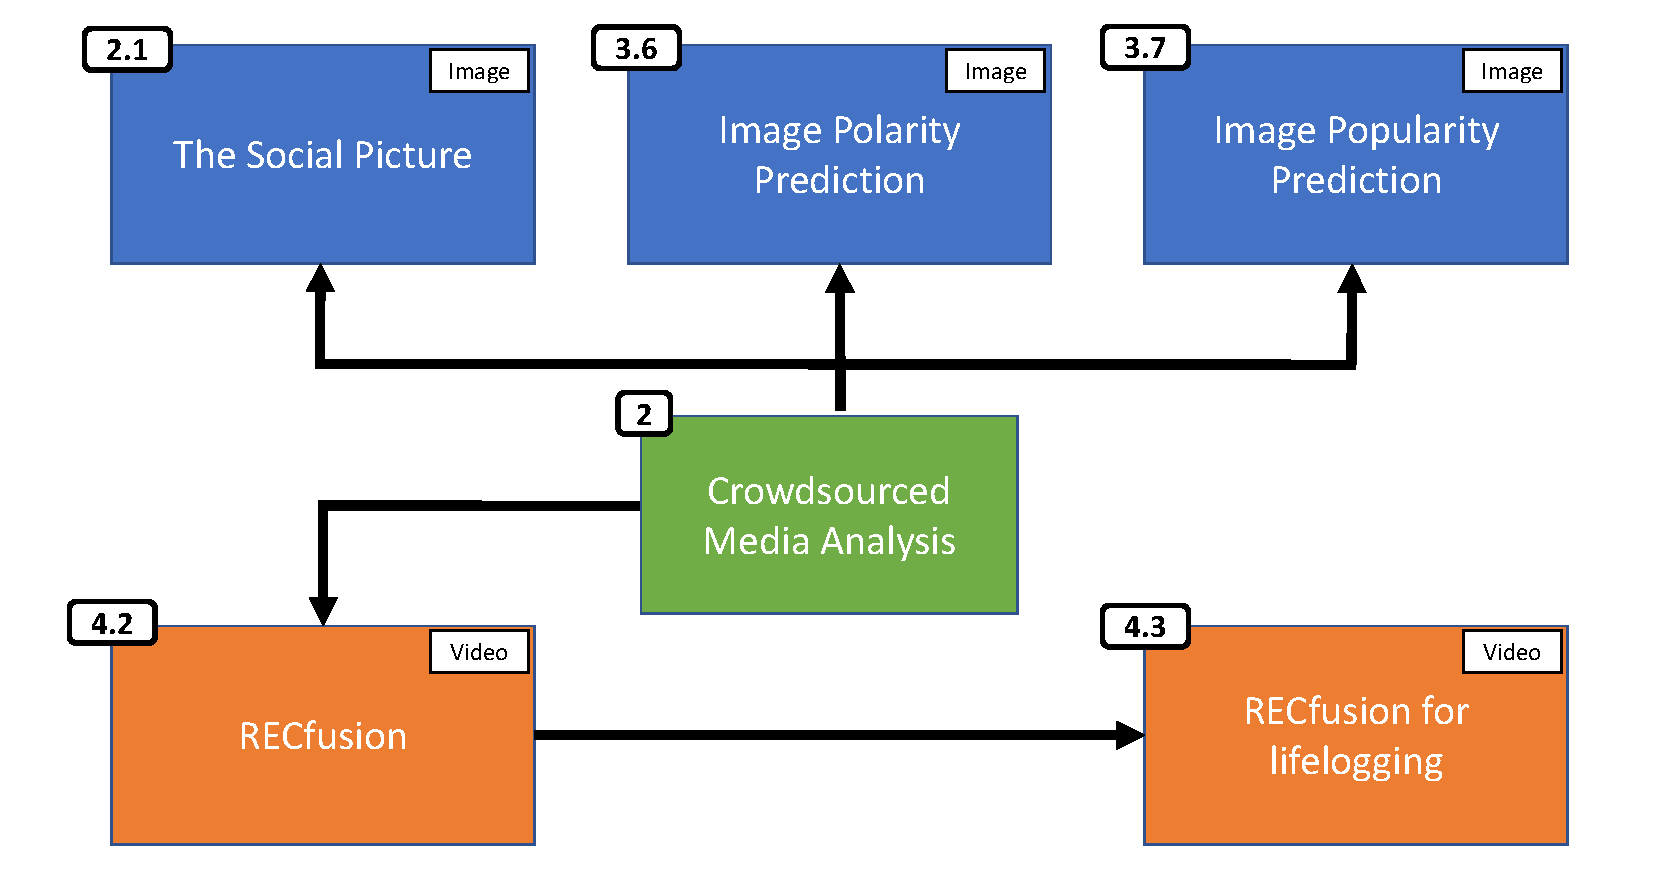
\includegraphics[width=1\linewidth]{schema.pdf}
	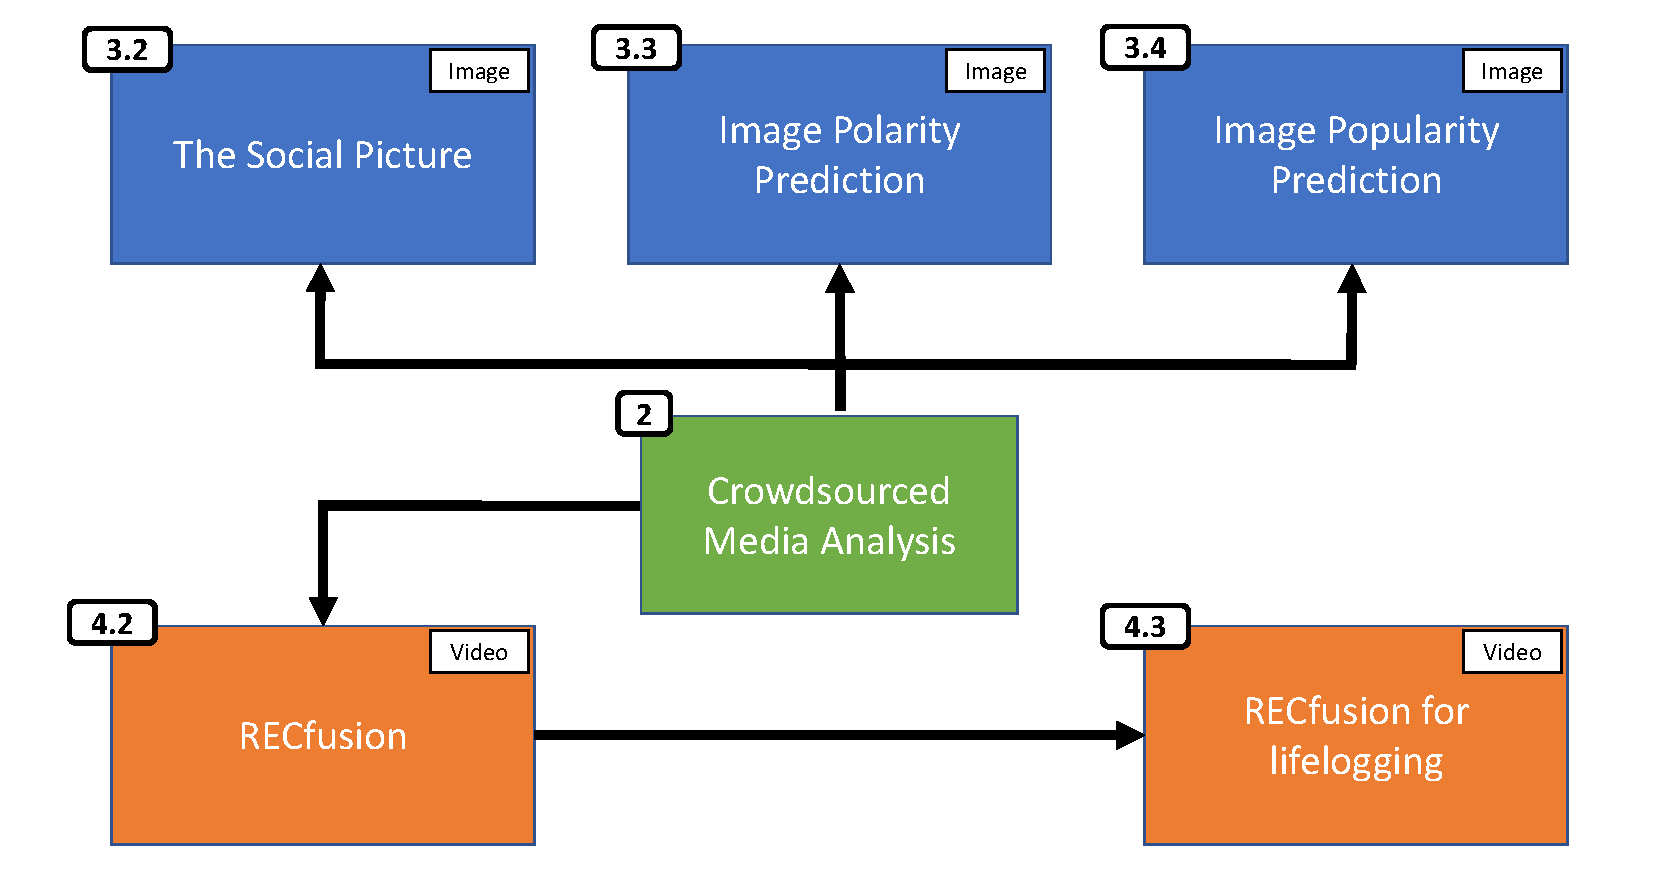
\includegraphics[width=0.8\linewidth]{schema2.pdf}
	\caption{Dissertation structure. Numbers depicts the Sections which describe the proposed work. Blue blocks represent algorithms that work on images, whereas orange blocks represent algorithms that work on videos. All the media involved in the works presented in this dissertation are produced by users or group of people with common interests (i.e., crowds).
	}
	\label{figDissertationSchema}
\end{figure}
In this dissertation, titled \virgolette{Methods for Sentiment Analysis and Social Media Popularity of Crowdsourced Visual Contents}, we mainly treated image and video contents produced by groups of users (i.e., crowdsourced).
For this reason, the dissertation is properly divided into three main parts: Crowdsourced Media Analysis, Image Sentiment Analysis and Video Sentiment Analysis.
The dissertation structure is shown in Figure~\ref{figDissertationSchema}. We start our discussion by an introduction on Crowdsourced Media Analysis, which brings together all the works presented in this dissertation. Each algorithm is presented in a different Section. In Chapter~\ref{ch3}, we present all the methods that analyses images for the tasks of users behaviour analysis, image polarity prediction and image popularity prediction.
In Chapter~\ref{ch4}, we present our works related to the analysis of video contents.
In this research work, the sentiment associated to images has been studied under several meanings. Hence, different research questions have been addressed. 
One is to understand the most popular subjects related to a place or an event, by the analysis of the images produced by users visiting that place or attending the event. This study produced two main framework: \textit{The Social Picture} and \textit{RECfusion}. The first framework is aimed to understand user preferences based on the pictures taken from users themselves in the context of a specific event or place. The output of \textit{The Social Picture} is a set of statistical insights about the collected images, as well as some exploration tools which allow to understand the most important subjects. The second is aimed to understand what is the scene recorded simultaneously by the most number of users attending the same event, based on the videos taken from the users at the same time. The output of \textit{RECfusion} is a video depicting the most popular scene over time composed by segments of videos selected from the users' ones.
The approach defined in \textit{RECfusion} has been further improved and extended to the First Person View (PFV) video domain, for the task of daily monitoring for assistive lifelogging.



\section{List of Publications}